\documentclass{article}

\usepackage{titlesec}
\usepackage{titling}
\usepackage[margin=1in]{geometry}
\usepackage{graphicx}

\titleformat{\section}
{\huge\bfseries\lowercase}{}{0em}{}[\titlerule]

\titleformat{\subsection}
{\bfseries\Large}{$\bullet$}{0em}{}

\titleformat{\subsubsection}[runin]
{\bfseries\large}{}{0em}{}[---]


\renewcommand{\maketitle}{
\begin{center}
{\huge\bfseries
\theauthor}

\vspace{.25em}
Software Analyse les 3
\end{center}
}

\begin{document}
\title{R\'esum\'e}
\author{Iljo De Poorter}

\maketitle
\section{activity diagram}
Kijk naar je use case, en bekijk waar het start.

Daar plaats je een bolletje

Daarna lopen we het normale verloop af, en plaatsen we dat in een rechte normale lijn. Elke keer dat de user iets doet moet het een activitiy(rechthoekje) zijn in je diagram. Eerst werk je met het normale verloop.

Daarna plaats je de post conditie

\begin{figure}[h]
  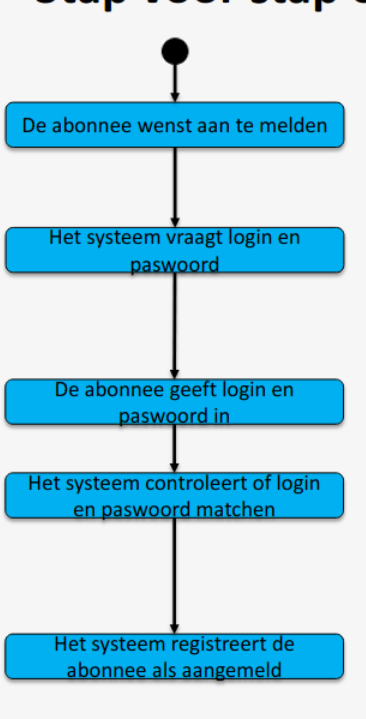
\includegraphics[width=0.2\linewidth]{boat.png}
\end{figure}

\subsection{Alternatieve verloop}

Eerst moet je analyseren waar het alternatief verloop start, in dit voorbeeld(zie slides) is dit vanaf stap 4.
Tussen stap 4 en 5 plaats je dan een ruit(disicion note)

Dan plaats je [geldig] bij het normale pad en [ongeldig] bij het alternatieve pad.

Uiteindelijk volgen we het hele alternatief pad en plaatsen we ook de plaats waar de alternatieve conditie uiteindelijk zal stoppen, (in dit geval tussen stap 1 en 2)

\begin{figure}[h]
  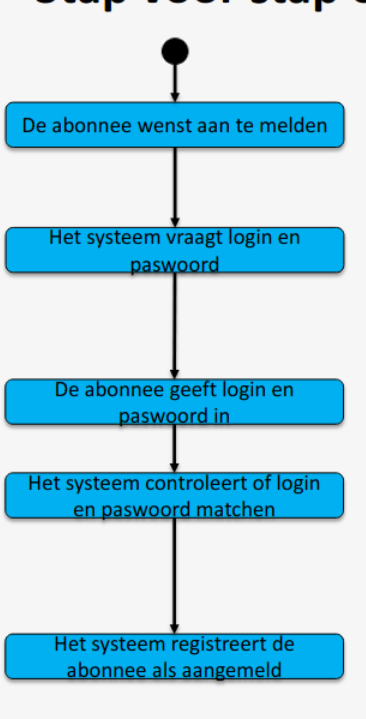
\includegraphics[width=0.2\linewidth]{boat.png}
\end{figure}

\section{Test scenario}

Op het moment dat de tester wilt starten met het "controleren" van het systeem, moet hij nadenken hoe hij dit wilt aanpakken. Dit zijn de test scenario's.

\subsection{Het belang van testen}
Je wil zeker zijn dat de software doet wat jij verwacht

Je wil kunnen aantonen dat er verwachtingen in functionaliteit geformuleerd zijn die moeten werken.

Het is belangerijk dat je maar 1 ding pre tijd test, dus als je een ongeldig passwoord ingeeft, zou je niet tegelijkertijd ook nog eens een ongeldige username moeten ingeven.
Daarna documenteer je ook goed wat er fout is gegaan, en wat er goed is gegaan. Het is ook van belang de verwachtingen op voorhand te formuleren.

\begin{figure}[h]
  \includegraphics[width=1\linewidth]{tests.png}
\end{figure}

In elk testscenario uit de use case wordt 1 testcase = minstens alle unieke wege uit het AD.
\end{document}
